This section will be a discussion on the architectural and design patterns to be employed in the Action Hero Defense game. There will be a presentation of the patterns to be used, explaining why the particular pattern was chosen and how we plan to implement it.

\subsection{Architectural pattern}
\subsubsection{MVC}
For the overall design of our application we have chosen the \textbf{Model-View-Controller} (MVC) pattern, which focuses on separating the domain, or application, logic of an application, from the user interface. It consists of tree different structures\cite{wiki:mvc}:
\begin{itemize}
\item \emph{Model} - responsible for managing the behavior of the system. This is where the main functionality and data management of the system should reside.
\item \emph{View} - typically the user interface of the system. Responsible only for drawing or displaying information on screen. The data which is supposed to be shown, is generated and managed in the model.
\item \emph{Controller} - manages input from the user in addition to what should be the following response from the system. An input may instantiate an action for either the model and/or view. 
\end{itemize}

 
A MVC-pattern provides several benefits. In our case the separation of domain logic and user interface provides a solid foundation for supporting the main quality attributes of our system; modifiability and testability. 

If we consider a model responsible for the core functionality of a system, the ability to add a new feature would mainly be concerned with the model of the system, limiting modification to only one module. This way we ensure a loose coupling between the different modules of the system, and thus making it easier to modify a single part of the system. In addition, the MVC-pattern could also help prevent ripple effects which can occur when a module is changed. A change in the user interface would not change anything in the model, and vice versa, a change in one of the methods of the models would not interfere with the user interface, as long as the method still returns the same type of value. 


The testability-aspect also benefits greatly of the isolation of domain logic, especially when considering unit testing of a system. A unit-test should not have to be concerned with what happens in the user interface, it should only focus on the behavior of the domain logic. What happens when a user press a button at the user interface should not be the unit tests responsibility. Tests concerning dependency and communication between modules would be more of an integration test's responsibility. 


With unit testing, the model will again be the main focus point. Unit test can be applied to only the model of the system. If a test would require user input to test a certain function, the tests-classes should be responsible for generating mock values to simulate user input. In this way, the functionality can easily be tested in isolation and with no dependency of the user interface. We should however assume that some form of design patterns and principles within the model are being practiced.


For our tower defense game, the MVC-pattern will be responsible for defining the architecture. The View of the software will be responsible for drawing and animation of the sprites and images on screen, whereas the controller will naturally be responsible for taking user input, and communicating this input to the view and model. The model will be responsible for monitoring and managing the status of both the game, the player and the enemies. The status of an enemy will for instance be changed when a cannonball hits the enemy, and the object, located in the model section,  responsible for monitoring the enemy's health status will be invoked. 

A (preliminary) concept of how the MVC-model should work in practice is as follows: an event, say a tower shoots at an enemy, will be first processed by the view which animates the particular event. As the cannonball-sprite collides with the enemy-sprite, a collision-event should occur. The collision detection would here be part of the controller, which then proceeds to invoke the model which in turn updates the enemy (and game) status. 
\subsection{Design Pattern}
\subsubsection{Singleton Pattern}
When implementing the Singleton design pattern, one restricts the instantiation of a class to one object. The purpose of this is to allow visibility for a class in the entire system. While the singleton pattern does not increase the modifiability, which is the main quality attribute the system is supposed to incorporate, it is important to keep track of the state of the system. The singleton pattern introduces many dangers, such as mutual dependencies, which usually increase the complexity of the system. It is important to maintain proper synchronization in a multi-threaded environment, with the introduction of Singleton pattern (global variables).

Singleton classes have few differences from a static class, but the main difference is that a Singleton class allows lazy initialization. Lazy evaluation is an evaluation strategy which allows a class to only initialize if needed. That way, resources may be saved. Resource usage is usually something which affects the performance quality attribute, which is not the main focus for this project. That aside, performance is still a factor which should not be ignored. \cite{wiki:singleton}

The different quality attributes affect each other, and some affect each other in negative way. In the case of Singleton pattern, which could be looked at a pattern increasing performance in many cases, it reduces modifiability, but increases performance.  

\subsubsection{Abstract factory}

\begin{figure}[h]
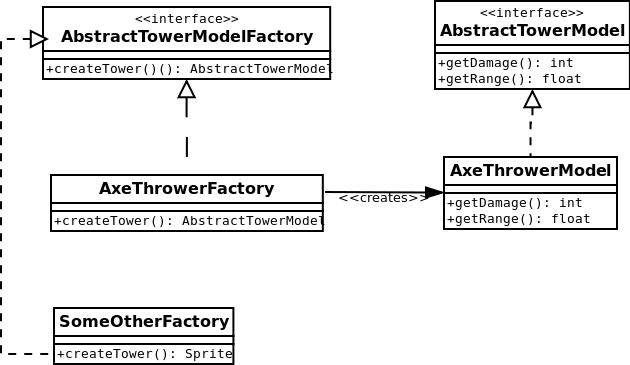
\includegraphics[width=1\linewidth]{images/abstractFactory.png}
\caption{Class diagram of the abstract factory pattern}
%\label{fig:absfac}
\end{figure}

The abstract factory pattern concerns the creation of objects. The main idea is that it provides an interface for the creation of related objects, without specifying the concrete classes. A normal way of incorporating this pattern would be to create a concrete implementation of an abstract factory, which creates concrete classes, and letting the client code be unaware of the concrete implementation, all it needs is an object implementing the abstract factory. \cite{wiki:abfac}  


In our case, the abstract factory would be useful when creating similar objects which will be in frequent use. An example of this is the sprites which will be displayed on the screen, for instance generating enemies. The enemy-objects could be similar, however with some unique properties. In this context an abstract enemy factory would seem like a good design solution. A diagram illustrating the concept is shown below:



We should here assume that we have a Sprite interface, an interface which we use to display all of the graphical objects on the screen. Relating it to the MVC, we could also assume that such a Sprite have a corresponding model-object, where we also could employ the abstract factory design pattern. 

As it stands, these are the main patterns we will focus on implementing to our Android game. 
